\documentclass[parskip=half]{scrartcl}
	
\usepackage[english]{babel}
\usepackage[latin1]{inputenc}
\usepackage{enumerate} % til \begin{enumerate}[(i)]
\usepackage{enumitem} % til at styre lister globalt
\usepackage{latexsym} % symboler
\usepackage{amsthm} % til thm osv
\usepackage{amssymb} % flere symbloer
\usepackage{bm} % bold math symbols
\usepackage{amsmath} % til pmatrix
\usepackage[hyphens]{url} %til \url med bindestreger
%\PassOptionsToPackage{hyphens}{url}\usepackage{hyperref}
\usepackage[pdftex]{graphicx}	
\usepackage{scrlayer-scrpage} % page setup
\usepackage[all,cmtip]{xy}

\usepackage{framed}
\usepackage[cache=false]{minted} % for source code
\usepackage{xcolor}
%set page header
\chead{FYS-STK4155 --- project 1}


% List will number things using (a), (b), ...
\setenumerate[1]{label={(\alph*)}} % Global setting

% Title setup
\title{Report for project 2}
\date{\today}
\author{Adam P W S{\o}rensen}

%%%%%%%%%%%%
% make chi subscripts low enough
% from http://tex.stackexchange.com/questions/191551/greek-chis-subscript-expressions-how-to-make-it-smaller-or-offset-lower
\let\latexchi\chi
\makeatletter
\renewcommand\chi{\@ifnextchar_\sub@chi\latexchi}
\newcommand{\sub@chi}[2]{% #1 is _, #2 is the subscript
  \@ifnextchar^{\subsup@chi{#2}}{\latexchi^{}_{#2}}%
}
\newcommand{\subsup@chi}[3]{% #1 is the subscript, #2 is ^, #3 is the superscript
  \latexchi_{#1}^{#3}%
}
\makeatother

\newcommand{\setof}[2]{\left\{ #1 \; \middle\vert \; #2 \right\}}

\DeclareMathOperator{\cspan}{\overline{span}}

% Theorem opsætning
\newtheorem{theorem}{Theorem}[section]
\newtheorem*{theorem*}{Theorem}
\newtheorem{lemma}[theorem]{Lemma}
\newtheorem{corollary}[theorem]{Corollary}
\newtheorem{proposition}[theorem]{Proposition}
\newtheorem{example}[theorem]{Example}
\newtheorem{conjecture}[theorem]{Conjecture}
\theoremstyle{definition}
\newtheorem{definition}[theorem]{Definition}
\newtheorem{assumption}[theorem]{Standing Assumption}
\newtheorem*{assumption*}{Standing Assumption}
\theoremstyle{remark}
\newtheorem{remark}[theorem]{Remark}
\newtheorem{notation}[theorem]{Notation}

%%%%%%%%%%%%
% notation short cuts
\newcommand{\vect}[1]{{\bm{#1}}}
\newcommand{\funcname}[1]{{\color{blue}{\texttt{#1}}}}
\newcommand{\varname}[1]{\texttt{#1}}
%%%%%%%%%%%%
% bb letters
\newcommand{\C}{\mathbb{C}}
\newcommand{\E}{\mathbb{E}}
\newcommand{\N}{\mathbb{N}}
\newcommand{\Q}{\mathbb{Q}}
\newcommand{\R}{\mathbb{R}}
\newcommand{\Z}{\mathbb{Z}}
% cal letters
\newcommand{\A}{\mathcal{A}}
\newcommand{\B}{\mathcal{B}}
\newcommand{\D}{\mathcal{D}}
\newcommand{\cL}{\mathcal{L}}
\newcommand{\M}{\mathcal{M}}
\newcommand{\cZ}{\mathcal{Z}}
% frak letters
\newcommand{\fA}{\mathfrak{A}}


%%%%%%%%%%%%%%
\begin{document}
%%%%%%%%%%%%%%

\maketitle

\begin{abstract}
We used neural networks for a regression and a classification problem. 
For our specific regression problem, the energy of a one dimensional ising system, we saw that linear regression ($MSE \approx 0$) did far better than the neural network ($MSE \approx 40$).
For the classification we looked at determining if a  two dimensional ising system was ordered or disordered. 
Here the neural network (accuracy $\approx 0.98$) did much better than logistic regression (accuracy $\approx 0.67$)
\end{abstract}


\section{Introduction}

The simplest form of a classification problem gives a set of data and then ask a yes-or-no question. 
If a persons liked \emph{The Fellowship of the Ring} and \emph{The Two Towers} will they then also like \emph{Return of the King}?
A more serious version provides weight, height, exercise level, dietary information and so on about a patient, and then ask if they will suffer from diabetes later in life. 

In many cases we probably prefer a probability that the answer is yes, over a simple yes or no answer. 
One way to achieve this is through logistic regression.
In logistic regression we look for a linear model that separates our data into two classes. 
For instance we might try to predict future diabetics as those with weight and sugar intake above some levels\footnote{This is very reductive view of diabetics}. 

Neural network offer a different path to classification and they can also be used for regression. 
Where the coefficients in linear and logistic regression offer insights into how parameters matter for the final answer, neural networks are more opaque. 
But they are also more powerful, at least in theory. 
The main point of this project is to use neural networks for regression and classification. 
When doing regression we compare our neural network to linear regression and for classification we compare it to logistic regression. 
We will do all our test on the so-called Ising model, using one dimensional data for the regression case and two dimensional data for classification. 

The Ising model is a famous model and used widely in science.
In the one dimensional case we will use regression to try to predict the energy of a system, and in two dimensions we will try to classify systems into ordered or disordered states.

We shall see that neural networks struggle with some linear regression problems. 
So much so, that if our data comes with a lot of structure, we probably better of not using neural networks.   
Linear regression will far out perform the networks for the one dimensional ising data. 

While neural networks are sure to have problems with certain classification task, in this project we will see them out preform logistic regression on the two dimensional ising data. 

\begin{framed}
All the code I have implemented can be found in the jupyter notebook \texttt{Projekt 2.ipynb} at \url{https://github.com/adam-wie/ml-exercises}.
A print of the jupyter notebook is uploaded along side this report.
\end{framed}

The report is structured as follows. 
In Section \ref{sec:methods} we will introduce, more rigorously, logistic regression and neural networks.
We will touch on their theory and how I have coded them.
In particular we will also discuss stochastic gradient descend. 
In Section \ref{sec:1dising} we use linear regression and neural networks to study the one dimensional ising data
And in Section \ref{sec:2dising} we use logistic regression and neural networks to study the two dimensional case. 
Finally in Section \ref{sec:conclusion} we summarize our findings.

\section{Methods} \label{sec:methods}
 
\subsection{Linear regression} \label{sec:linear} 

The three linear regression methods I have used - ordinary least squares regression, ridge regression, and lasso regression - are discussed in detail in the report for project 1.
In short, each data point is a row vector $\vect{x}_i$ of features, each has a corresponding measured value $z_i$, and the goal is to find a column vector $\vect{\beta}$ such that 
\[
	\begin{pmatrix}
		\vect{x_1} \\
		\vect{x_2} \\
		\vdots \\
		\vect{x_n}
	\end{pmatrix} \vect{\beta}
	\approx
	\begin{pmatrix} z_1 \\ z_2 \\ \vdots \\ z_n \end{pmatrix}.	
\] 

Let us now zoom in on an import distinction between the way linear regression methods and neural networks were used for regression in this project.  
Suppose we are preforming a biology experiment.
For each test person we record their height and weight and perform a measurement of their cholesterol level. 
Now the question is if height and weight somehow can predict cholesterol level. 
Using linear regression we now have to decide on a model.
Do we think cholesterol can be predicted simply by height and weight, or do we need more features like powers of height and weight and products of these powers. 
Perhaps we could even consider using Body Mass Index (BMI) (it appears that there is in fact some correlation between BMI and cholesterol levels \cite{somepaper}).
Each of these choices will lead to different models we have to choose between.
But in each case the coefficients will give an indication of how much each future matters.
This is a real strength of linear regression methods. 

In contrast to this, as we will discuss below, when we do neural networks, we aim to find a network configuration that can be trained to give good predictions when we feed in height and weight. 
And it can be quite daunting to review the networks weights and biases to deduce how each feature contributes.     

\subsection{Stochastic gradient descend} \label{sec:sgd}

For both logistic regression and neural network we will use a version of stochastic gradient descend. 
Stochastic gradient descend is a methods for minimizing functions.
To explain how we will use it, first we fix some notation. 
Suppose we are given some (training) data in the form of matrix $X$ and the corresponding true predictions $\vect{y}$. 
Each row $\vect{x}_i$ of $X$ is one data point. 
Suppose further that our model makes prediction based on some parameters $\vect{\beta}$, denote the prediction $P(X, \vect{\beta})$. 
If we have a cost function $C$ that determines how good our predictions are, then we want to choose $\vect{\beta}$ to minimize $C(\vect{y}, P(X, \vect{\beta}))$.   
With $X$ and $\vect{y}$ fixed, this is only a function of $\vect{\beta}$. 
We can use the stochastic gradient descend method, then there is some function $c$ such that 
\[
	C(\vect{y}, P(X, \vect{\beta})) = \sum_{i=1}^N C(\vect{y}_i, P(\vect{x}_i, \vect{\beta})).
\] 
Note that this is the case if our cost function is a sum of squares, and it also holds if it is the cross entropy. 

To do a non-stochastic gradient descend method, fix a learning rate $\eta$. 
If our current guess for a minimum of $C(\vect{y}, P(X, \vect{\beta}))$ is $\beta_0$, then a single step of gradient descend updates that guess to 
\[
	\beta_{1} = \beta_0 - \eta \nabla C(\vect{y}, P(X, \vect{\beta})) \vert_{\beta = \beta_0}
\]
where $\nabla C(\vect{y}, P(X, \vect{\beta})) \vert_{\beta = \beta_0}$ denotes the gradient of $C$ evaluated at $\beta_0$.

For stochastic gradient descend, the only difference is that each update of $\beta$ is only based on part of the training data. 
First the training data is randomly split into mini batches $X_1, X_2, \ldots, X_n$.
We split on data points, not features, and each mini batch should consist of roughly the same number of data points. 
The true values are split up in the same way as $\vect{y}_1, \vect{y}_2, \cdots, \vect{y}_n$.
If our current choice of parameters is $\beta_0$, then for $i = 1,2, \ldots, n$ we let 
\begin{align*}
	\beta_i &= \beta_{i-1} - \eta \nabla C(\vect{y_i}, P(X_i, \vect{\beta})) \vert_{\beta = \beta_{i-1}}, \\
			&= \beta_{i-1} - \eta E \left[ \nabla c(y_k, P(\vect{x}_k, \vect{\beta})) \vert_{\beta = \beta_{i-1}})\right].
\end{align*}
Here $E[ \cdots ]$ denote the average of the gradients of $c$, each computed by using one row $\vect{x}_k$ in $X_i$, and its corresponding true value $y_k$.  

The point of stochastic gradient descend is that if we use $m$ batches, then we get to update our guess of $\beta$ $m$-times, for each pass we make over the training data. 
Which should speed up convergence. 

This is implemented as follows in the code:

\begin{minted}{python}
####
# This function does one sgd using batches to find a min.
# X is the input data
# ys are the true output values
# dcost is the derivative of the cost function of a sinlge data point
# learning_rate is the learning rate
# bs is the batch size, which must divide the number of data points
def sgd_bathces_min(X, ys, dcost, epochs, learning_rate, bs = 1) :
    N = len(ys) # number of data points
    m = N//bs # number of batches
    p = X.shape[1] # number of columns in X, i.e. number of parameters
    theta = np.random.uniform(-0.7, 0.7, (p, 1)) 
    
    for epo in range(epochs)  :
        # shufffel the row index and reshape
        batches = np.random.permutation(N).reshape((-1, m)) 
        for batch in batches :
                # compute the gradient for each row in the batch, 
                # and stack them together
                grad_matrix = \
                np.hstack([dcost(X[b].reshape(-1,p), ys[b], theta) for b in batch])
                # avarage the entries of each row 
                # we also need to make sure numpy thinks of grad as a column vector
                grad = np.mean(grad_matrix, axis=1).reshape(p,-1)

                theta = theta - learning_rate * grad
        
     return theta
\end{minted}

In terms of implementation there some book keeping to make sure that all vectors are of the right shapes, but most of the work are in computing \varname{grad\_matrix} and \varname{grad}. 
To compute \varname{grad\_matrix} we build one derviate for each data point in the batch , which we then combine with \funcname{np.hstack}. 
By taking means, we get \varname{grad}. 
This computation of \varname{grad\_matrix} is somewhat general, as it really only needs to know how to compute the derivative of a single row. 
On the other hand, for our purposes it is probably quite inefficient, as we do not take advantage of a matrix multiplication to compute many gradients at once.  

I could not find sci-kit learn functionality to directly compare my code to. 
Part of the problem being that there are a lot of random choices involved.
In the code block title \emph{Comparing my sgd to sci-kit learn}, I compare a simple linear regression solved using stochastic gradient descend from sci-kit learn and the one from my code. 
I get slightly different coefficients (on the 3rd decimal), but they are close enough for me to believe it all works.  

\subsection{Logistic regression} \label{sec:logistic} 

Logistic regression is used when the goal is to classify some data in to two groups. 
When training a classification model, each training data point is given by a row vector $\vect{x}_i$, and a correct classification $t_i \in \{0,1\}$.  
Given some unknown data vector $\vect{x}$, instead of doing a hard prediction of $0$ or $1$, we will instead predict a value $p \in [0,1]$. 
The idea is that $p$ is the probability that $\vect{x}$ should be classified as $1$. 
The theoretical description of logistic below build on \cite{Ng}.

Before providing details about logistic regression we fix some notation. 
We let $\sigma \colon \R \to \R$ be the sigmoid function given by 
\[
	\sigma(x) = \frac{1}{1 + \exp(-x)}.
\]
This function is also called the logistic function, which is probably where the name logistic regression comes from. 
Note that $0 < \sigma(x) < 1$ for all $x \in \R$ but that $\sigma(x) \to 1$ as $x \to \infty$ and $\sigma(x) \to 0$ as $x \to -\infty$. 
It is worth observing that $\sigma$ is increasing on all of $\R$.
If $A$ is a matrix and $f$ is a function we will use numpy notation and write 
\[
	f(A) = 
	f \left(  \begin{pmatrix} a_{11} & a_{12} & \cdots \\ a_{21} & a_{22} & \cdots \\  \vdots & \vdots & \ddots \end{pmatrix}	 \right)
	= \begin{pmatrix} f(a_{11}) & f(a_{12}) & \cdots \\ f(a_{21}) & f(a_{22}) & \cdots \\  \vdots & \vdots & \ddots \end{pmatrix}.
\]
We will mostly use this when $A$ is a vector. 

Logistic regression is very similar to linear regression. 
Suppose our data point has $p$ features, i.e. are represented by row vector of size $p$. 
Then we are again searching for a column vector $\vect{\beta}$ of size $p$, and our prediction for a data point vector $\vect{x}$ is $\sigma(\vect{x} \vect{\beta})$.
Hence, if we are given a training set $\setof{ \vect{x}_i}{i = 1,2, \ldots, N}$ with corresponding classifications $\setof{z_i}{i = 1,2,\ldots, N}$ we define the design matrix $X$ and a vector $\vect{z}$ by   
\[
	X = \begin{pmatrix}
	 \vect{x}_1 \\
	 \vect{x}_2 \\
	 \vdots \\
	 \vect{x}_N	
	 \end{pmatrix}, 
	 \quad \text{ and } \quad
	 \begin{pmatrix}
	 z_1 \\ z_2 \\ \vdots \\ z_N
	\end{pmatrix},
\]
and try to find $\vect{\beta}$ such that 
\[
	\sigma(X \vect{\beta}) \approx \vect{z}.
\]

We measure closeness of our predicted probabilities not using mean squared error, but rather the cross entropy. 
Given a vector of predictions $\vect{p}$ and a vector of true values $\vect{z}$, both of size $N$, we define the cross entropy, $\ell$, as 
\[
	\ell(\vect{z}, \vect{p}) = - \sum_{i=1}^N \left( z_i \ln(p_i) + (1-z_i) \ln(1 - p_i)  \right).
\]
Note that $z_i \in {0,1}$, so each term in the sum is either $\ln(p_i)$ or $ln(1-p_i)$. 
That is, each term in the sum is the natural logarithm of the probability that we assign to the right answer.
If that probability is close to one, we get a very small contribution to the sum, if it is close to zero, we get a very large (negative) contribution. 

As discussed in project 1, we can also define a cost function that penalizes the size of the parameters. 
So we could do a ridge version of logistic regression. 
For this we fix a regularization parameter $\lambda$, and then try to find the $\beta$ that minimizes the cost function given by
\[
 \text{Cost}(\beta) = \ell(\vect{z}, \sigma(X \beta)) +  \lambda \sum_{j=1}^p \beta_j^2.
\]
To find $\beta$ we use stochastic gradient descend. 
 
Logistic regression is implemented in the code block under the heading \emph{Logistic Regresion}.
The implementation is just a class that does a call to my stochastic gradient descend method when it is fit. 
The derivative of a single row of data is given by 
\begin{minted}{python}
def diff_ce_ridge(xs, y, b0, alpha) :
    return (sigmoid(xs @ b0)-y)*(xs.T) + 2*alpha*b0
\end{minted}
Note that this derivative is slightly different than the one found in \cite{Ng}, since there they aim to maximize $-\ell$.

To test that the regression works, I did a small test in the code block under the heading \emph{Test of my logistic regression}.
Here we use the moons data set from sci-kit learn and compare a logistic regression performed by sci-kit learn and by my method. 
As for the linear regression case, we do not get exactly the same coefficients, with more of a difference this time. 
But if we look at the accuracy of the two methods they are the same, and ``by eye'' the decision boundaries look very similar.   

\subsection{Neural networks} \label{sec:neuralnet} 
 
Neural networks can be quite complicated. 
To give a simple introduction we will restrict to the case of an input layer with one node, a single hidden layer with $n$ nodes, and an output layer with a single note.
Diagrammatically we have this setup.
\[
	\xymatrix{
		& & \text{input} \ar[drr] \ar[dr] \ar[d] \ar[dl] \ar[dll] & &  \\
		\circ \ar[drr] & \circ \ar[dr] & \cdots \ar[d] & \circ \ar[dl] & \circ \ar[dll] \\
		& & \text{output} & & 
	}
\]
Each arrow is then assigned a weight. 
Let us denote the weights out of input by $\alpha_1, \alpha_2, \ldots, \alpha_n$, and the weights into output by $\beta_1, \beta_2, \ldots, \beta_n$. 
Each neuron in the hidden layer needs an activation function, here we will pick the sigmoid function, and we will use a linear output.
What all this means, is that if $N$ denotes the function that given an input $x$ computes the output of the neural network, then $N$ has the form:
\[
	N(x) =  \sum_{i=1}^n \beta_i \sigma(\alpha_i x).
\]  
 
When using a neural networks to approximate some function $f$, we then aim to choose the weights and activation function such that $N(x) \approx f(x)$. 
One can show that using the setup described above that is in fact possible in almost all imagianable situations \cite{Hornik}.  
The tricky part is how to train the network. 

Training of neural networks is done using a technique known as back propagation.
We will follow the theory is laid out in \cite[Chapter 2]{Nielsen}. 
However, as one can see from the code, I chose to use row vectors for data points, but it Nielsen (and most everyone else it seems) uses columns. 
There is no real difference in the formulas, just a few transposes. 
I made my choice to match with what we did for logistic and linear regression, but in retrospect it was a bad choice. 

At its heart the back propagation algorithm is a gradient descend method. 
Denote our cost function by $C$ and assume it has the form $C(X, \vect{y}) = \sum_{i} c(\vect{x_i}, y_i)$. By clever use of the chain rule, one can compute expressions that let us compute $\frac{\partial C}{\partial \alpha_i}$ and $\frac{\partial C}{\partial \beta_i}$ relatively efficiently. 
If we are in the simple setting described above, that is not too bad to do by hand, but if we include biases, and especially more hidden layers, it becomes a mess.

For my implementation I chose to have each layer be a class, and then a network class contains a list of layers. 
I restricted myself to the situation where there is a single output neuron, since that is all we need, and it made the partial derivatives a little easier to implement. 
My back propagation follows the recipe at the end of \cite[Chapter 2]{Nielsen} very closely.
Here is the code for updating the weights given a batch of data:

\begin{minted}{python}
def one_step_back_propagate(self, batch, learning_rate, dsummand) :
	batch_size = batch.shape[0] # number of rows in batch
	deltas = [] # list of deltas, build starting from the back
        
	# first feed forward to compute as and zs
	acts, zs = self.feed_forward(batch)

	# Compute deltas, according to formulas from Nielsen's boook
	# http://neuralnetworksanddeeplearning.com/chap2.html
	# Since each delta only depends on the previously computed delta, 
	# we use pythons -1 indexing
        
	# First we define the final delta 
	deltas.append(dsummand(acts[-1])*self.doutact(zs[self.number_of_layers]))
	deltas[-1].reshape(1,-1)
	# then each is defines using the previously computed 
	for layer, z in zip(self.layers[-1::-1], zs[-2:0:-1]) :
    	deltas.append((deltas[-1] @ layer.weights.T)*self.dhact(z))
                        
	# Now update the weights and biases
	# We go through the layers and activations from behind, 
	# we do not consider the final activation, as that does not appear in the formulas 
	# We use of np.mean for the bias update but not for the weights, 
	# due to the way matrix multiplication works, (1/batch_size) * (a.T @ delta)
	# is the average row_of_a.T @ row_of_delta (as they run over all row).
	# For the biases we need forcefully take the avarage
	for layer, a, delta in zip(self.layers[::-1], acts[-2::-1], deltas):
    	layer.weights = layer.weights - (learning_rate/batch_size) * (a.T @ delta)
	    layer.bias = layer.bias - learning_rate * np.mean(delta, axis=0)
\end{minted}  

The final for loop is very similar to what we saw for stochastic gradient descend. 
Every thing before just uses the back propagation equation to compute all derivatives. 

Fortunately for me, someone wrote a very nice piazza note on how to check that back propagation works. 
In the code block under the heading \emph{Comparing our backpropagation algorithm to sci-kit learn}, I implemented these checks, and it all works out. 
In order to do the checks one needs the various gradients, which my methods do not return. 
But simply by setting the learning rate and batch sizes to 1, one can deduce them as the change in weights and biases.    

The code blocks under the headings \emph{A simple test of the mean square version of the network} and \emph{Testing the corss entropy version of the network} just tries the network with different activation and cost functions on some toy problems. 
It does not really provide a whole lot of information, I was just excited to see my hard work do something!

For the activation functions I have implemented the relu and sigmoid functions (also the linear function, but that is only for outputs), and I have either cross entropy as cost or square sums.  

I have not been able to find good sources for how more neurons in layer or more hidden layers impact a neural network. 
It seems that the network becomes harder to train with more layers and neurons, but potentially also more powerful. 
In the one input and one output case, the network function $N$ is just a real valued function. 
If we use relu as the activation function we can say a little bit. 
Here $N$ is piecewise linear and has (at most) as many break points as there are hidden neurons. 
   
\section{1 dimensional Ising data (parts b and d)} \label{sec:1dising}

I have used linear regression and neural networks to try to model the one dimensional ising data. 
This is all done in the code blocks following the heading \emph{1D Ising model data}. 
For the linear regression I used the build in functions from sci-kit learn, as the code I had written for project 1, was specialized to the setting from project 1. 
I did import my cross validation and bias variance codes.  

Since there is no noise in our observations the standard OLS regression gives a perfect model. 
However, my bias and variance computations show that neither vanish, which I cannot quite explain. 

For both ridge and lasso we use cross validation to pick the penalty parameter, and then do bias and variance estimates. 
There is no bias for the lasso model and only very little variance. 
For the ridge model we get bias and variance close to that of normal linear regression. 
The most interesting thing about these computations is how they weight each coupling, this is shown in the following heat maps.

\begin{figure}[H]
\caption{Weight to each coupling in OLS, rigde, and lasso regression.}
\centering
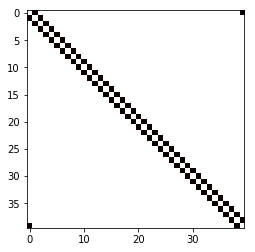
\includegraphics[scale=0.4]{ols.png}
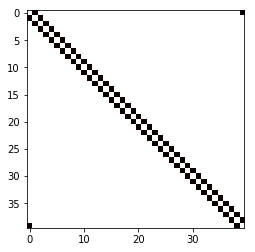
\includegraphics[scale=0.4]{ridge.png}
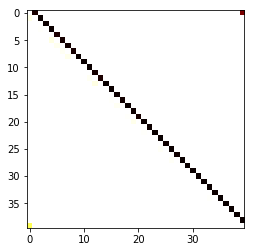
\includegraphics[scale=0.4]{lasso.png}
\end{figure}

What is noticeable about this, is that the OLS and ridge regression distribute the power of the coupling between two states $i$ and $i+1$ evenly into the $(i, i+1)$ and $(i+1, i)$ entries. 
Whereas the lasso puts it all in $(i, i+1)$. 
The difference between ridge and lasso is downto how they regularize, but it is not clear to me why OLS favours one over the other.  

When using the neural net, I chose a model with a single hidden layer, and sigmoid as the activation function of the hidden layer. 
I varied the learning rate and number of neurons, then tested the trained networks to pick the best model. 
The following figure summarizes these test,

\begin{figure}[H]
\caption{Choosing network setup.}
\centering
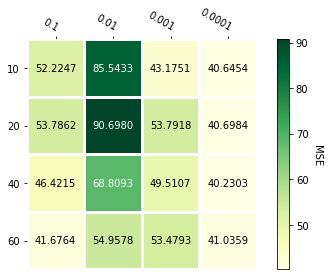
\includegraphics[scale=0.6]{1disingneurons.png}
\end{figure}

No configuration gives a truly spectacular mean squared error, but the best seems to have $40$ hidden neurons and a learning rate of $0.0001$. 
I trained that net over a larger set of epochs, 500, but did not see an improvement of mean squared error. 
In fact, one some runs the error went up a little bit, which I suspect is due to the randomness inherited to the methods.    

\section{2 dimensional Ising data (parts c and e)} \label{sec:2dising}

I tried different learning rates and regularization parameters to find the best choice for logistic regression. 
These are summarized in the following figure.

\begin{figure}[H]
\caption{Choosing logistic setup.}
\centering
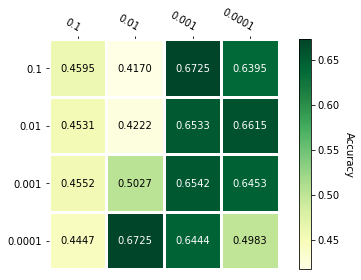
\includegraphics[scale=0.6]{2dlogistic.png}
\end{figure}

We see that one of the best models has a learning rate of $0.001$ and a regularization of $0.1$. 
Training this model for more epochs I didn't get the accuracy beyond $0.67$. 

For the neural network we again decided on single hidden layer, with both hidden and output activation functions being sigmoid. 
Using different configurations of the network, we found the following accuracies. 

\begin{figure}[H]
\caption{Choosing logistic setup.}
\centering
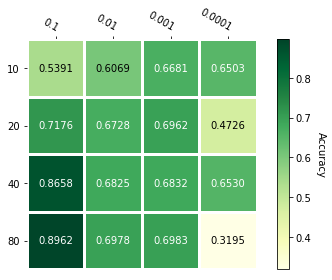
\includegraphics[scale=0.6]{2dnet.png}
\end{figure}

The best result came with a $80$ hidden neurons and a learning rate of $0.1$. 
Training that model for more epochs, we got the accuracy upto $\approx 0.98$.

The size of the 2d ising files were such that running these test where painful for my laptop. 
Given infinite time and computing power, I should very much have liked to try out other configurations. 
In particular, it is sometimes mentioned as a rule of thumb, that the hidden layer should have half as many neurons as there are inputs. 
But testing with 800 hidden neurons is beyond me and my laptop. 
It would also be nice to try with deeper networks with more hidden layers, even if it seems unlike to improve our results.   

\section{Conclusions (part f)} \label{sec:conclusion}

We found the linear regression ($MSE \approx 0$) far out performed neural networks ($MSE \approx 40$) on the one dimensional ising data. 
Furthermore, from the coefficients from linear regression, we are able to read of the constant $J$, but have no such avenue for neural networks. 

I suspect the neural networks poor performance is to do with the fact that it is famously hard (\cite{xor}) to train neural networks to solve XOR. 
The one dimensional ising model seems very closed to just a collection of XORs. 

For the classification problem we saw that a neural network (accuracy $\approx 0.98$) outdid logistic regression (accuracy $\approx 0.67$). 
This must mean that the 2 dimensional ising states are not linearly separated. 
Other than that, it is hard to draw other conclusions than that it is exciting to see the power of neural networks. 


%%%%%%%%%%%%%%
%Bibliography
\bibliographystyle{apalike}
\bibliography{refs}	% expects file "refs.bib"
%%%%%%%%%%%%%%


\end{document}